\documentclass[polish,aspectratio=169]{beamer}

% wide screen
% \documentclass[aspectratio=169]{beamer}


%%% YOUR PACKAGES HERE %%%
\usepackage{comment}
\usepackage{hyperref}
\usepackage[backend=biber, style=numeric, bibstyle=ieee,
            sorting=none, isbn=false, urldate=ymd,
            doi=false, url=true]{biblatex}
\addbibresource{bibliography/bibliography.bib}
\renewbibmacro{in:}{}
\usepackage{subfigure}
\usepackage{graphicx}
\usepackage{geometry}
\usepackage{float}
\usepackage{listings}
\usepackage{xcolor}

\newcommand{\refrys}[1]{Rys.~\ref{#1}}
\newcommand{\reflist}[1]{List.~\ref{#1}}
\newcommand{\refEq}[1]{Równ.~\ref{#1}}
% \usepackage{tikz} 
% \usetikzlibrary{graphs,graphs.standard,automata}


\definecolor{keywordcolor}{rgb}{0.1,0.1,0.8}
\definecolor{stringcolor}{rgb}{0.7,0.1,0.1}
\definecolor{commentcolor}{rgb}{0.3,0.7,0.3}
\definecolor{backgroundcolor}{rgb}{0.95,0.95,0.95}
\lstdefinelanguage{FSharp}{
    keywords={let, match, with, in, function, if, then, else, rec, type, module, open},
    keywordstyle=\color{keywordcolor}\bfseries,
    sensitive=true,
    comment=[l][\color{commentcolor}\itshape]{//},
    morecomment=[s][\color{commentcolor}\itshape]{(*}{*)},
    string=[b]",
    stringstyle=\color{stringcolor},
    basicstyle=\ttfamily,
    numbers=left,
    numberstyle=\tiny\color{gray},
    backgroundcolor=\color{backgroundcolor},
    showstringspaces=false
}
% polish language
\usepackage[polish]{babel}
\usepackage{polski}



%%% IMPORT PG PRESENTATION STYLE %%%
% THIS IS GDANSK UNIVERSITY OF TECHNLOGOGY (PG) PRESENTATION TEMPLATE
% Creator: Jan Cychnerski <jan.cychnerski@eti.pg.edu.pl>
% Copyleft 2019


% PG THEME OPTIONS

\usetheme{Boadilla}
\usecolortheme{default}
\usefonttheme{professionalfonts}

% colors

\definecolor{PGBlue}{RGB}{0,56,101}
\definecolor{PGRed}{RGB}{193,10,39}
\definecolor{PGSilver}{RGB}{200,200,200}
\definecolor{PGBlack}{RGB}{0,0,0}

% PGBlue
\setbeamercolor{frametitle}{fg=PGBlue}
\setbeamercolor{normal text}{fg=PGBlue}
\setbeamercolor{structure}{fg=PGBlue}
\setbeamercolor{item}{fg=PGBlue}

% PGRed
\setbeamercolor{alerted text}{fg=PGRed}
\setbeamercolor{item projected}{fg=PGRed}

% white
\setbeamercolor{title}{fg=white}
\setbeamercolor{titlelike}{fg=white}
\setbeamercolor{subtitle}{fg=white}

% enumerate and itemize styles

\setbeamertemplate{itemize item}{\bfseries\color{PGRed}\raise1pt\hbox{\donotcoloroutermaths$\bullet$}}
\setbeamertemplate{itemize subitem}{\color{PGRed}\raise0.5pt\hbox{--}}
\setbeamertemplate{itemize subsubitem}{\color{PGRed}\tiny\raise1.5pt\hbox{\donotcoloroutermaths$\bullet$}}

\setbeamertemplate{enumerate item}{\bfseries\color{PGRed}\insertenumlabel.}
\setbeamertemplate{enumerate subitem}{\color{PGRed}\insertsubenumlabel.}
\setbeamertemplate{enumerate subsubitem}{\color{PGRed}\insertsubsubenumlabel.}
\setbeamertemplate{enumerate mini template}{\insertenumlabel}


% disable navigation

\beamertemplatenavigationsymbolsempty

% additional commands

\newcommand*{\vcenteredhbox}[1]{\begingroup
\setbox0=\hbox{#1}\parbox{\wd0}{\box0}\endgroup}

\graphicspath{{pgbeamer/}}


\usepackage{iflang}
\IfLanguageName{polish}{
\newcommand{\pglogobig}{pg-logo-big-pl}
\newcommand{\pglogosmall}{pg-logo-small-pl}
}{
\newcommand{\pglogobig}{pg-logo-big-en}
\newcommand{\pglogosmall}{pg-logo-small-en}
}


% FRAME TITLE LOGO
\addtobeamertemplate{frametitle}{\vcenteredhbox{\includegraphics[height=8mm]{\pglogosmall}}\bfseries}{}


\newcommand{\pgtitleframe}{{
% PG TITLE PAGE

\setbeamercolor{background canvas}{bg=PGBlue}
\setbeamercolor{title}{fg=white}
\setbeamercolor*{date}{fg=white}
\setbeamercolor*{author}{fg=white}

\setbeamertemplate{footline}{}

\begin{frame}[noframenumbering]
\centering
\vspace{1cm}
\includegraphics[height=3cm]{\pglogobig}
\vspace{5mm}
\maketitle
\end{frame}
}}

\newcommand{\pglastframe}{{
% PG LAST PAGE

\setbeamercolor{background canvas}{bg=PGBlue}
\setbeamercolor{title}{fg=white}
\setbeamercolor*{date}{fg=white}
\setbeamercolor*{author}{fg=white}

\setbeamertemplate{footline}{}

\begin{frame}[noframenumbering]
\centering
\vspace{1cm}
\includegraphics[height=5cm]{\pglogobig}
\end{frame}
}}



%%% YOUR OPTIONS HERE %%%

\title[Property based testing]{Property based testing}
\subtitle{Jak testować zachowanie, a nie przypadki}
\author{Paulina Brzęcka \and Marek Borzyszkowski}
\date{\today}

\setbeamercovered{transparent}

\begin{document}
%%% PG TITLE PAGE %%%
\pgtitleframe

%%% YOUR PRESENTATION HERE %%%

\setbeamercovered{invisible}

\begin{frame}{Wstęp}
    Istnieje wiele koncepcji testowania oprogramowania, jedną z nich jest testowanie na podstawie właściwości \cite{pbt_bib}.
    \onslide<2->{Dziś dowiecie się:
        \begin{enumerate}
        \item na czym polega testowanie na podstawie właściwości.
        \item Czym różni się ono od klasycznego podejścia do testowania.
        \item Jakie są strategie testowania na podstawie właściwości. 
        \item Jak przy wykorzystaniu konceptu QuickCheck znaleźć wartości początkowe nieprzechodzące testy.
        \end{enumerate}
    }
\end{frame}

\begin{frame}{Przykład}
    TODO
\end{frame}

\begin{frame}{Strategie}
    Testowanie na podstawie właściwości nie jest proste w zastosowaniu, przynajmniej przy pierwszej próbie.
    Istnieją jednak pewne schematy wskazujące drogę, jak stworzyć takie testy.
    \begin{enumerate}[<+->]
        \item Różne ścieżki, ten sam wynik
        \item Tam i z powrotem
        \item Są rzeczy niezmienne
        \item Z czasem rzeczy przestają się zmieniać
        \item Dziel i rządź
        \item Łatwiej zweryfikować niż zaimplementować
        \item Testowanie z wyrocznią
    \end{enumerate}
\end{frame}

\begin{frame}{Strategie - Różne ścieżki, ten sam wynik}
    \begin{columns}[t]
        \column{.5\textwidth}
            Jedną z podstawowych strategii skorzystanie z komutatywności niektórych operacji. Można to zrobić poprzez wykonanie operacji w różnej kolejności.\\
            \onslide<2->{
                Przykładem takiej strategii może być komutatywność dodawania z 
                % \reflist{kod:add_all_properties}
                , gdzie wykorzystano \texttt{add x y}, jak i odwrotność tej operacji \texttt{add y x}.\\ 
            }
            \onslide<3->{
                Innym przykładem jest test metody \texttt{sort} danej listy. 
                Wykonanie sortowania, a następnie dodanie do każdego elementu listy \texttt{1} powinno dać taki sam efekt jak dodanie \texttt{1} do każdego z elementów listy, a następnie jej posortowanie \refrys{fig:commutative_strategy_list_sort} %\reflist{kod:list_sort_add1}.
            }
        \column{.5\textwidth}
        \centering
        \begin{figure}
            \centering
            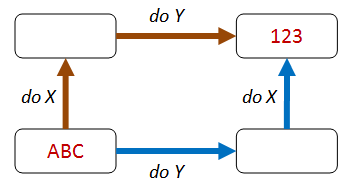
\includegraphics[width=1\textwidth]{images/property_commutative.png}
            \caption{Strategia - komutatywność}
            \label{fig:commutative_strategy}
        \end{figure}    
    \end{columns}
\end{frame}

\begin{frame}{Strategie - Tam i z powrotem}
    \begin{columns}[t]
        \column{.5\textwidth}
            Przykładem takiego testu mogą być przeciwne operacje matematyczne jak:
            \begin{itemize}[<+->]
                \item \texttt{dodawanie/odejmowanie}
                \item \texttt{mnożenie/dzielenie}
                \item \texttt{potęga/logarytm}.
            \end{itemize} 
            \onslide<4->{Innymi przykładami są operacje niekoniecznie matematyczne:}
            \begin{itemize}[<+->]
                \item \texttt{serializacja/deserializacja}
                \item \texttt{zapis/odczyt z pliku}
                \item \texttt{wstaw/sprawdź czy zawiera}.
                \item \texttt{odwrócenie listy/odwrócenie listy}
            \end{itemize} 
        \column{.5\textwidth}
        \centering
        \begin{figure}
            \centering
            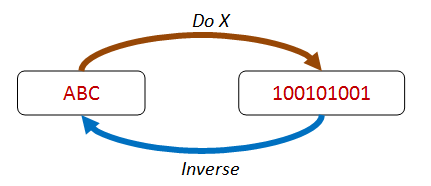
\includegraphics[width=1\textwidth]{images/property_inverse.png}
            \caption{Strategia - inwersja}
            \label{fig:inverse_strategy}
        \end{figure}    
    \end{columns}
\end{frame}

\begin{frame}{Strategie - Są rzeczy niezmienne}
    \begin{columns}[t]
        \column{.5\textwidth}
            Czasami testowana funkcja przetwarzając dane zachowuje część ich właściwości \refrys{fig:invariant_strategy}.
            Chociażby funkcje \texttt{sort} lub \texttt{map} wykonane na liście \texttt{n} elementów, zwracaja odpowiednio zmodyfikowaną listę \texttt{n} elementową.
        \column{.5\textwidth}
        \centering
        \begin{figure}
            \centering
            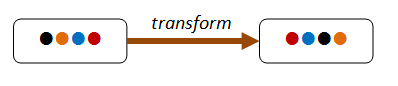
\includegraphics[width=1\textwidth]{images/property_invariant.png}
            \caption{Strategia - niezmienność}
            \label{fig:invariant_strategy}
        \end{figure}    
    \end{columns}
\end{frame}


\begin{frame}{Strategie - Z czasem rzeczy przestają się zmieniać}
    \begin{columns}[t]
        \column{.5\textwidth}
            Inną właściwością funkcji może być niezmienność wyniku funkcji po ponownym jej zaaplikowaniu \refrys{fig:independance_strategy}. 
            Innymi słowy, wykonanie funkcji 2 razy daje taki sam efekt, jak jednokrotne jej zaaplikowanie.
            \onslide<2->{Przykładami takich operacji, dla których taki typ testu miałby zastosowanie to metoda \texttt{distinct} wykonana na danej liście, lub wykonanie \texttt{update} na danej bazie danych.            }
        \column{.5\textwidth}
        \centering
        \begin{figure}
            \centering
            
\includegraphics[width=1\textwidth]{images/property_idempotence.png}
            \caption{Strategia - idempotentność}
            \label{fig:independance_strategy}
        \end{figure}    
    \end{columns}
\end{frame}


\begin{frame}[fragile]{Strategie - Dziel i rządź}
    \begin{columns}[t]
        \column{.5\textwidth}
            Istnieją sposoby na testowanie na podstawie właściwości jest wykorzystanie rekursywności struktur przekazywanych do funkcji, takich jak \texttt{listy}, \texttt{drzewa} \refrys{fig:recursive_strategy}. 
            \onslide<2->{
                Przykładem może być sprawdzenie za pomocą tej metody funkcji sort \reflist{kod:list_sort_rec}.\\
                \texttt{TU WSTAWIĆ LISTING}
                % \lstset{language=FSharp, basicstyle=\scriptsize}
                % \begin{lstlisting}[frame=single,caption={Test sortowania listy z wykorzystaniem strategii rekursywnej},label=kod:list_sort_rec]
                % let rec firstLessThanSecond_andTailIsSorted sortFn (aList:int list) =
                % let sortedList = aList |> sortFn
                % match sortedList with
                % | [] -> true
                % | [first] -> true
                % | [first;second] -> first <= second
                % | first::second::rest->
                %     first <= second &&
                %     let tail = second::rest
                %     // check that tail is sorted
                %     firstLessThanSecond_andTailIsSorted sortFn tail
                % \end{lstlisting}
            }
            \column{.5\textwidth}
        \centering
        \begin{figure}
            \centering
            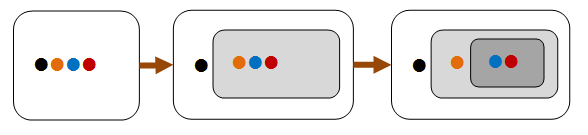
\includegraphics[width=1\textwidth]{images/property_induction.png}
            \caption{Strategia - rekursywność}
            \label{fig:recursive_strategy}
        \end{figure}    
    \end{columns}
\end{frame}


\begin{frame}{Strategie - Łatwiej zweryfikować niż zaimplementować}
    \begin{columns}[t]
        \column{.5\textwidth}
            Niekiedy testowana funkcja jest skomplikowana, ale jej rezultat da się łatwo sprawdzić. Przykładem może być funkcja wyszukująca wyjście z labiryntu \refrys{fig:easy_verification_strategy}, gdzie sam algorytm wyszukiwania odpowiedniej ścieżki jest skomplikowany, 
            natomiast samo sprawdzenie, czy ścieżka dobrze prowadzi do wyjścia można w łatwy sposób zweryfikować.
        \column{.5\textwidth}
        \centering
        \begin{figure}
            \centering
            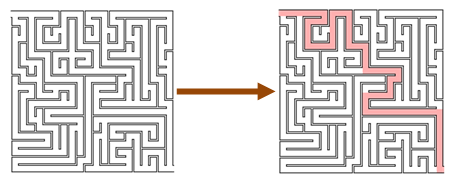
\includegraphics[width=1\textwidth]{images/property_easy_verification.png}
            \caption{Strategia - łatwe sprawdzenie}
            \label{fig:easy_verification_strategy}
        \end{figure}    
    \end{columns}
\end{frame}


\begin{frame}{Strategie - Testowanie z wyrocznią}
    \begin{columns}[t]
        \column{.5\textwidth}
            Zdaża się, że funkcjonalność została już napisana i trzeba ją zrefactorować, przepisać, napisać od nowa \refrys{fig:oracle_strategy}. Warto wtedy wykorzystać wartości zwracane przez oryginalnie zaimplementowany algorytm jako pewną wartość wyniku, pewnego rodzaju wyrocznię, uznając go jako prawdę. 
            W taki sposób można sprawdzić, czy nowa funkcja w pewnym stopniu pokrywa się ze starą funkcją. Czasami też istnieje wiele algorytmów doprowadzających do tego samego wyniku, mające różne złożoności, czy też działające równolegle. 
            Można wykożystać wtedy najprostrzy algorytm jako wyrocznię, ze względu na najmniejsze prawdopodobieństwo napisania takiego algorytmu z błędem. Następnie, przy wykorzystaniu wyroczni, stworzyć bardziej skomplikowany (często efektywniejszy) algorytm.
        \column{.5\textwidth}
        \centering
        \begin{figure}
            \centering
            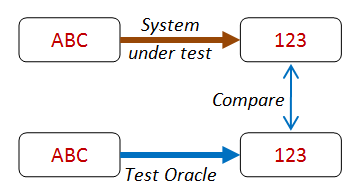
\includegraphics[width=1\textwidth]{images/property_test_oracle.png}
            \caption{Strategia - wyrocznia}
            \label{fig:oracle_strategy}
        \end{figure}    
    \end{columns}
\end{frame}

\begin{frame}{Pytania}
    \begin{center}
        {\huge Pytania?}
    \end{center}
\end{frame}

\setbeamercovered{transparent}
\begin{frame}[allowframebreaks]{Bibliografia}
    \printbibliography
\end{frame}

\begin{frame}{Podziękowania}
    Chcielibyśmy podziękować Panu dr. inż. Janowi Cychnerskiemu za stworzenie 
    i udostępnienie stylu \href{https://github.com/jachoo/pg-beamer}{\emph{pg-beamer}}, 
    co zostało wykorzystane do stworzenia tej prezentacji.\\
    \url{https://github.com/jachoo/pg-beamer}
     
\end{frame}

\begin{frame}{Koniec}
    \begin{center}
        {\huge Dziękujemy za uwagę!}
    \end{center}
\end{frame}

%%% PG LAST PAGE %%%
\pglastframe


%%% DOCUMENT ENDS HERE. Good bye! :) %%%

\end{document}
